%*****************************************************************************
	\chapter{Analysis and design of the solution}
	Based on the assignment I hit into a question \emph{How should the dialogue with a blind pedestrian look like?} After hours spent thinking about how to do it. I was advised from my supervisor just to observe. So I did. I used an iterative technique, where I started analysing dialogue of two people and ended up with a fully standalone web app.
	\section{Natural dialog human-2-human over a map}
	\label{sec:FirstExperiment}
	I started with a game. It was a two player game. One player was simulating a \emph{\uv{blind} user} walking in a city the second player was seeker. I was playing the \emph{seeker}, asking the user questions and trying to localize him.
	
	%todo image
	\begin{figure}[h]
		\centering
		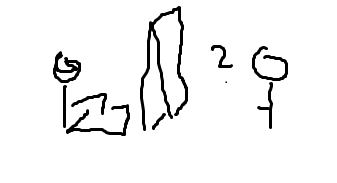
\includegraphics[width=0.7\linewidth]{figures/1stExp-human2humanOverMap/bigpicture}
		\caption[Setup]{}
		\caption{}
		\label{fig:bigpicture}
	\end{figure}

	These game sessions were recorded and then analysed. The analysis shown the \emph{topics} and \emph{questions}, which was repeating. And could be used for an automated dialogue system.
	
	
	\paragraph{\uv{blind} user}
	The user was given the map and a piece of paper with cut out hole. See \ref{fig:map-and-blind-simulator}. The map was depicting all the enviroment: inclination of sidewalks, pedestrian crossings,  marking for blinds, rails, houses, parked cars, noises form cars, ticking noises from trafic lights, direction of cars, tram lines.
	
	The user choosed a place on a side walk he liked and put a cut out hole on that spot. Then he was responding the seekers questions, moving and exploring the environment based on seekers orders.
	
	\paragraph{seeker}
	The seeker had another copy of the map. He was asking the \emph{\uv{blind} user} questions and giving him orders. \uv{Do you have there buildings?}, \uv{Which hands do you have the house on?}, \uv{Are you going up hill?}. 
	Depending on the response i.e \uv{I am going downhill.} He was eliminating all the not suitable places (uphills, and horizontal sidewalks). When the possible space on the sidewalks narrowed to one point the seeker anouced \uv{Found you, you are here!} and showed it to the \uv{blind} user.
	
	\begin{figure}[h]
		\centering
		\includegraphics[width=0.7\linewidth]{"figures/1stExp-human2humanOverMap/map and blind simulator"}
		\caption[Map and blind simulator]{A map and paper with cutout hole, to simulate blind person and space he can explore}
		\label{fig:map-and-blind-simulator}
	\end{figure}
	\begin{figure}[h]
		\centering
		\includegraphics[width=0.7\linewidth]{"figures/1stExp-human2humanOverMap/using blind simulator"}
		\caption[User session]{A user is moving on the map and answering the questions of the facilitator}
		\label{fig:user-session}
	\end{figure}
	
	\paragraph{outputs}
	I was collecting all the answers the \emph{seeker} used. Then I clustered these questions accroding the topic and selected the most representative answer for each topic.
	
	\paragraph{testing details}
	Five friends interacted as users in this study. 3 mens and 2 womens. They were between 21 and 53 years old. Each participant went over 4 maps with consequently growing complexity of the environment.

	
	
	
	%todo picture of questions and answer
	\begin{figure}[h]
		\centering
		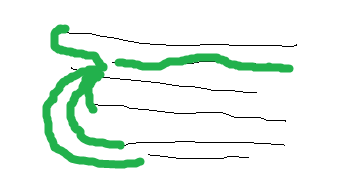
\includegraphics[width=0.7\linewidth]{figures/1stExp-human2humanOverMap/clusteredquestions}
		\caption[Best question for each topic]{}
		\caption{}
		\label{fig:clusteredquestions}
	\end{figure}
	
	The topics and the questions were
	\begin{itemize}
		\item \emph{Orders} - Describe where you are? Is there anything else interesting?
		\item \emph{Houses} - Do you have houses?
		\item ...
		%todo complete list
	\end{itemize}
	
		
	\section{Fixed questions human-2-WizzardOfOzz over a map}
	As a second step I built a low fidelity prototype of dialogue system. I wanted to verify the questions from the first experiment would work even when read aloud by a computer system and to see how the interaction would change.
	
	 I used Axure\cite{axure} to create a diagram and craft the logic of this system. And I used the Accapela text to speech (TTS) service\cite{accapela} to prerecord all seeker's questions and possible answers. So whenever I clicked on a field in the diagram, the computer read it alloud.
	 
	  I repeated the game from the first experiment, but this time the seeker was asking his questions based on the diagram logic, and as a response clicking on correct answer and leting it be read aloud by the machine voice.
	 
	 %todo fix images dialogue + largerimage of dialogue
\begin{figure*}[h]
	\centering
	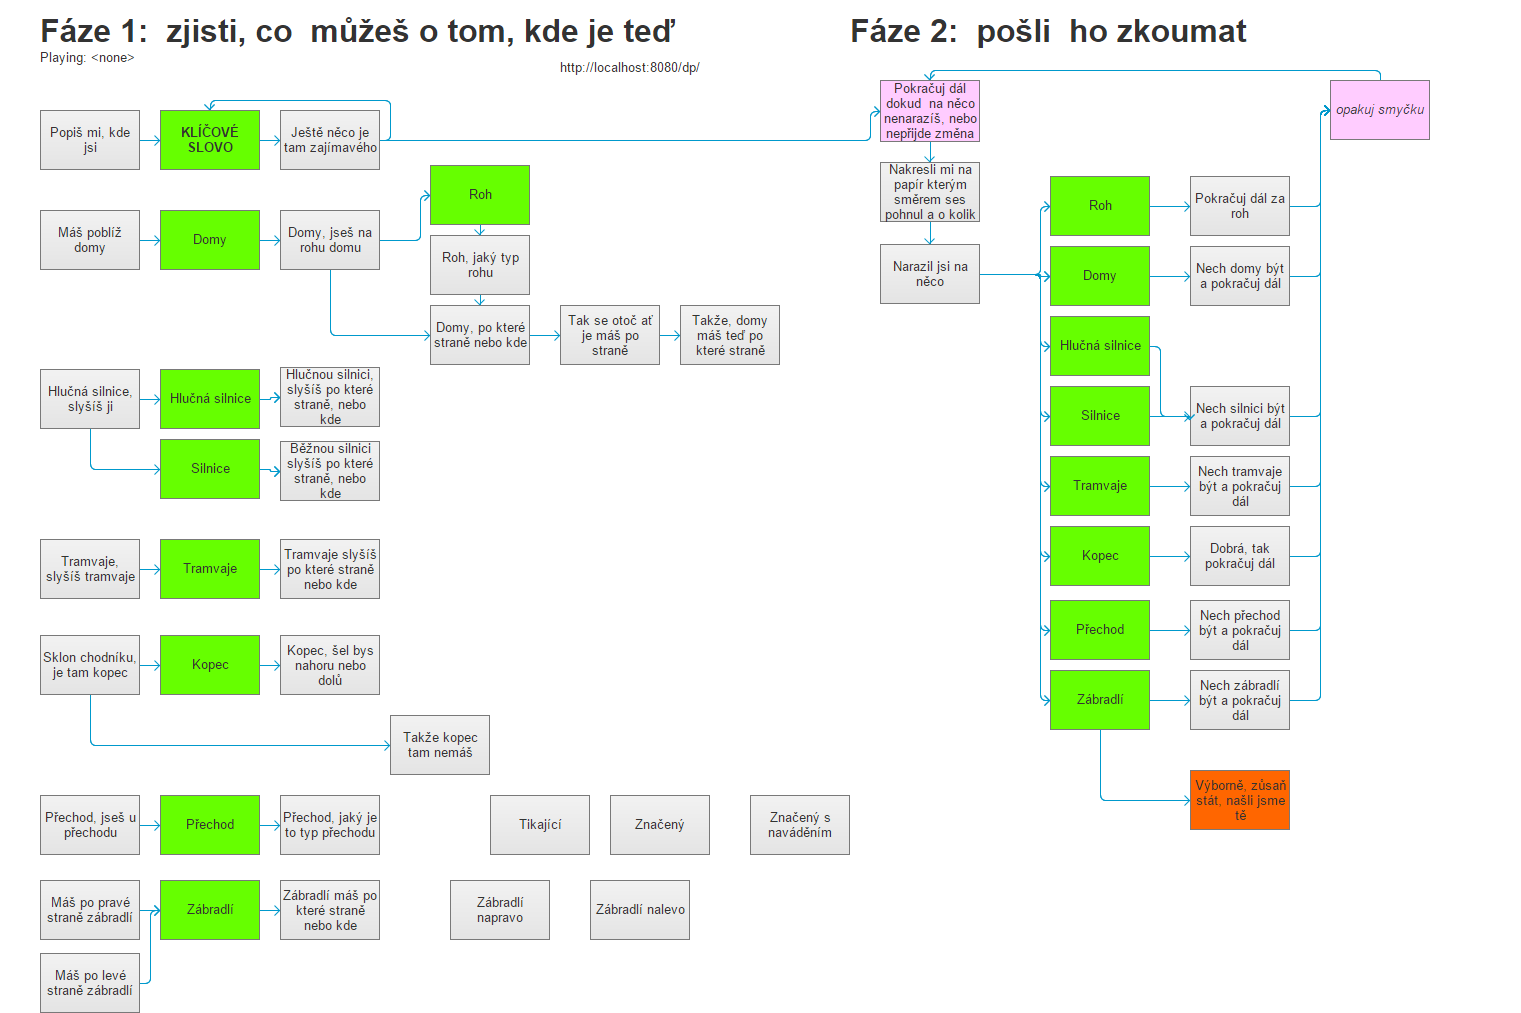
\includegraphics[width=0.7\linewidth]{figures/2ndExp-human2WoZOverMap/tested-dialogue}
	\caption[Dialogue]{}
	\caption{}
	\label{fig:tested-dialogue}
\end{figure*}


\begin{figure}[h]
	\centering
	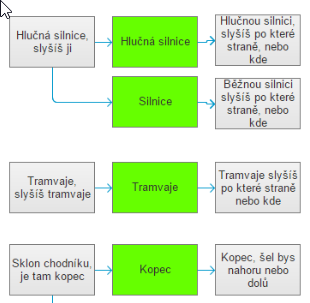
\includegraphics[width=0.7\linewidth]{figures/2ndExp-human2WoZOverMap/detail}
	\caption[Detail]{}
	\caption{}
	\label{fig:detail}
\end{figure}

\paragraph{outcomes}
I noticed the participants started to talk a lot woth one world setneces like \uv{yes}, \uv{uphill} or at least make very short senteces. All the richness of ansewers disappeared and the answers started to be very similiar between the participants. So when someone would give you the anonymised transcript, you could even recognize if it is from one person or not.
Next I evaluated the usability and comed up with a list of usability mistakes and errors in the possible ansers and minor dialogue issue in structure.

\paragraph{participants}
Another set of 5 friends of mine participated. Their age ranged from ? to ?. ? mens and ? womens. They again went as wall throught the same 4 maps with increasing complexity

	
	 I 
	\section{Fixed question human-2-WizzardOfOzz in the city}
	\section{Dialog system blind-2-WizzardOfOzz in the city}
	From the second and thir experiment I learned that it's sometimes impossible to decide the possition of person, it takes long and is error prone. And as well I compared it with the Naviterier data structure \cite{naviterier-data}. 
	%todo how it was exactly, what do i need
	I realised that most of the needed infos like trams, type of corners, altitude are not present in the API, thus not able to be used in a standallone application.
	
	And I started to play with Idea, do we even need it, can we just smartly use the data from the GPS, or utilize a person just hopped of the tram he knows the number and knows the stop?
	
	I came up with five prototypes. 
	
	\paragraph{POI}
	\paragraph{POI - with GPS}
	\paragraph{Crossing of two streets}
	\paragraph{GPS & compass}
	\paragraph{GPS wo compass}
	
	
	This time the Wizzard of Oz simulation went even further. The user was given a phone. And instructed, when he taps the upper part of the screen it means button one, lower part means button two. In fact the phone was turned off. The researcher was standing nearby and deterining the dialog again by clicking and leting the computer read aloud the TTS texts.
	
	\paragraph{outputs}
	
	https://docs.google.com/document/d/1xfWjAOKCVGUYHrUM910tLNwEvJqrzqakL6JYwVVPzdc/edit
	
	
	 
	\section{Hifi system blind-2-cell phone in the city}
	The last iteration brought three prototypes: \reversegeo, \gps and \poi. All three of them are fully working. The users can interact with them in the browser